%%%%%%%%%%%%%%%%%%%%%%% file main.tex %%%%%%%%%%%%%%%%%%%%%%%%%
%
% Revised manuscript for RAIRO - Operations Research
%
\documentclass{ro}
%
%%%%%%%%%%%%%--PREAMBLE--%%%%%%%%%%%%%%%%%%
\usepackage{graphicx}
\usepackage{algorithm}
\usepackage{algorithmic}
\usepackage{mathtools}
\usepackage{url}
\usepackage{xcolor}
\usepackage{enumerate}
\usepackage{ctable}
\usepackage{booktabs}
\usepackage[utf8]{inputenc}
\usepackage{amsmath}
\usepackage{amssymb}
\usepackage{float}
\usepackage{placeins}
\usepackage{multirow}
\usepackage{lineno}

\DeclarePairedDelimiter{\ceil}{\lceil}{\rceil}
\DeclarePairedDelimiter{\floor}{\lfloor}{\rfloor}
\newcommand\numberthis{\addtocounter{equation}{1}\tag{\theequation}}

\allowdisplaybreaks
\begin{document}

%%-----------------------------
%%      Top Matter
%%-----------------------------
\title{Dynamic ICU Bed Allocation Under Resource Scarcity: A Discrete-Event Simulation Integrating Multi-Type Beds and Triage Policies}

\author{Carlos Eduardo Veras Gomes}\address{Universidade Federal do Maranh\~ao, S\~ao Lu\'is, MA, Brazil.}\email{carlos.evg@dicente.ufma.br}
\author{Jo\~ao Augusto Ferreira Nunes de Carvalho}\address{Universidade Federal do Maranh\~ao, S\~ao Lu\'is, MA, Brazil.}\email{augusto.joa@dicente.ufma.br}
\author{Francisco Glaubos Nunes Cl\'imaco}\address{Universidade Federal do Maranh\~ao, Av. dos Portugueses, 1966, S\~ao Lu\'is, MA, Brazil.}\thanks{Corresponding author: francisco.glaubos@ufma.br}

\date{\today}

\begin{abstract}
During public health crises and epidemic surges, healthcare systems face acute shortages of Intensive Care Unit (ICU) beds, requiring transparent, ethically sound, and operationally rigorous allocation mechanisms. Previous optimization models have predominantly relied on static, one-shot allocations, overlooking critical temporal dynamics such as stochastic patient arrivals, variable length of stay (LOS), and patient deterioration while awaiting care in queues. This paper proposes a dynamic discrete-event simulation (DES) framework for multi-type ICU bed allocation (adult, pediatric, and neonatal) under scarce resources. The model is parameterized using verified operational bed capacities from the University Hospital of the Federal University of Maranh\~ao (HU-UFMA, CNES 2024; 45 specialized beds: 15 adult, 10 pediatric, and 20 neonatal). We evaluate four competing triage policies: Maximizing Overall Survival Expectation (MGS, prioritizing marginal survival gain), Least Serious First (LSF), Most Serious First (MSF), and First-Come, First-Served (FCFS) under a Common Random Numbers (CRN) paired experimental design over a 60-day continuous horizon. The results demonstrate that under low-demand conditions ($\rho = 0.7$), all policies achieve equivalent survival rates ($p > 0.05$). However, under severe surge capacity ($\rho = 1.6$), the MGS policy saves on average an additional $33.67$ lives over the standard FCFS hospital baseline ($t = 71.68, p < 0.0001$) and $16.78$ lives over the MSF heuristic, while reducing average queue waiting times from $33.1$ hours to $24.1$ hours. These findings provide actionable operational insights for hospital directors and triage committees in managing constrained critical care resources.
\end{abstract}

\subjclass{90B06, 90B15, 90B90, 92C50}
\keywords{Healthcare Operations Research; ICU Bed Allocation; Discrete-Event Simulation; Triage Policies; Multi-Type Critical Care Beds; Queueing Theory}

\maketitle

%%-----------------------------
%%      Main Text
%%-----------------------------

\section{Introduction}
\label{sec:intro}

Intensive Care Units (ICUs) represent the most resource-intensive and critical bottleneck in modern healthcare systems. When demand surges dramatically---as witnessed during the COVID-19 pandemic, severe respiratory illness seasons, or mass casualty events---ICU capacity is rapidly overwhelmed, forcing clinicians and healthcare administrators to confront harrowing triage decisions \cite{grasselli2020critical, aquino2022ethical}. In such scarcity contexts, traditional First-Come, First-Served (FCFS) admission is known to be sub-optimal, as it allocates life-saving beds without considering clinical prognosis, survival probabilities, or the potential years of life saved \cite{craxi2020rationing, dieteren2022should}.

To address this challenge, operations research and mathematical programming methodologies have emerged as central tools for designing rational allocation protocols \cite{dantzig2002linear, wolsey2020integer, frej2021decision}. Recently, \cite{frej2023collaborative} proposed an expected utility and Bayesian decision framework to allocate beds during acute crises, using the Sequential Organ Failure Assessment (SOFA) to quantify prognosis. Similarly, multi-principle frameworks \cite{White_2021} and capacity planning models \cite{Alban_2020, Schmidt_2021} have sought to rationalize admission rules.

However, existing literature exhibits a significant methodological gap regarding the **temporal dimension and decision timing** in actual ICU operations:
\begin{enumerate}[(i)]
    \item **Static vs. Dynamic Allocation:** Many mathematical models assume a static, one-shot batch problem where a fixed list of patients is allocated simultaneously to available beds. In reality, ICU decisions are inherently continuous and dynamic: patients arrive stochastically across shifts, occupy beds for variable lengths of stay (LOS), and depart through clinical recovery, transfer, or death \cite{Bilbao_2022, Valeva_2023}.
    \item **Patient Heterogeneity and Bed Specialization:** Critical care beds are not fungible commodities. A neonatal ICU (NICU) bed cannot accommodate an adult respiratory failure patient, nor can specialized pediatric ICU (PICU) teams manage adult multi-organ failure. Triage policies must account for segregated multi-type bed pools.
    \item **Queueing Delays and Reneging:** When all beds of a given specialty are fully occupied, arriving patients must wait in emergency or transitional wards. If waiting times exceed clinical tolerance thresholds, the patient's condition may irreversibly deteriorate or lead to pre-ICU mortality \cite{king2019modelling, Murray_2023}.
\end{enumerate}

To bridge this gap, this paper introduces a discrete-event dynamic simulation (DES) framework for multi-type ICU bed allocation under resource scarcity. Our study makes three main contributions:
\begin{itemize}
    \item **Realistic Temporal Decision Modeling:** We formulate a continuous-time simulation with Poisson arrival processes, stochastic log-normal bed occupancy durations (LOS), and finite queue tolerances (reneging), linking triage decisions directly to bed discharge epochs.
    \item **Multi-Type Critical Care Structure:** The model incorporates specialized bed categories (adult, pediatric, and neonatal) under exclusive clinical compatibility constraints, parameterized using verified public data from the National Register of Healthcare Establishments (CNES 2024) for the University Hospital of the Federal University of Maranh\~ao (HU-UFMA).
    \item **Rigorous Paired Policy Comparison:** We execute a Common Random Numbers (CRN) simulation across 100 replications over a 60-day horizon, comparing Maximizing Overall Survival Expectation (MGS), Least Serious First (LSF), Most Serious First (MSF), and FCFS across four levels of systemic demand intensity ($\rho \in \{0.7, 1.0, 1.3, 1.6\}$).
\end{itemize}

The remainder of this article is structured as follows. Section \ref{sec:works} reviews related literature and synthesizes existing approaches. Section \ref{sec:modeling} formalizes the mathematical and dynamic simulation model. Section \ref{sec:experiments} details the parameter calibration and experimental design based on HU-UFMA data. Section \ref{sec:results} discusses the simulation findings, paired differences, and queue dynamics. Finally, Section \ref{sec:conclusion} concludes with operational recommendations and directions for future research.

\section{Related Work}
\label{sec:works}

The management of ICU bed capacity and patient scheduling has attracted extensive investigation in healthcare operations research. Table \ref{tab:lit_comparison} provides a systematic comparative summary of key literature in relation to our work.

\begin{table*}[t]
\centering
\caption{Systematic comparison of the proposed model with existing ICU allocation and triage literature.}
\label{tab:lit_comparison}
\resizebox{\textwidth}{!}{
\begin{tabular}{lcccccc}
\toprule
\textbf{Study} & \textbf{Decision Horizon} & \textbf{Bed Types} & \textbf{Arrival Process} & \textbf{Length of Stay (LOS)} & \textbf{Queue / Reneging} & \textbf{Triage Criteria} \\
\midrule
Alban et al. \cite{Alban_2020} & Dynamic & Single & Poisson & Empirical / Erlang & Yes (Overflow) & Capacity threshold \\
Frej et al. \cite{frej2021decision} & Static & Single & None & None & No & Utility / Monte Carlo \\
White et al. \cite{White_2021} & Static & Single & None & None & No & Multi-principle scoring \\
Schmidt et al. \cite{Schmidt_2021} & Multi-period & Regional & Aggregate & Deterministic & No & Regional balancing \\
Bilbao et al. \cite{Bilbao_2022} & Dynamic & Single & Non-homog. Poisson & Phase-type & Yes & Admission / Early discharge \\
Dieteren et al. \cite{dieteren2022should} & Survey / Scenario & Single & None & None & No & Public preferences \\
Valeva et al. \cite{Valeva_2023} & Dynamic & Step-down & Markovian & Exponential & Yes (Beds blocking) & Acuity-based outflow \\
Frej et al. \cite{frej2023collaborative} & Static & Single & None & None & No & SOFA / Bayesian Utility \\
Murray et al. \cite{Murray_2023} & Dynamic & Single & ARMA Time-Series & Survival Analysis & No & Prognostic prediction \\
\textbf{This Work} & \textbf{Dynamic (DES)} & \textbf{Multi-type (3)} & \textbf{Continuous Poisson} & \textbf{Log-Normal Stochastic} & \textbf{Yes (Clinical timeout)} & \textbf{MGS, LSF, MSF, FCFS} \\
\bottomrule
\end{tabular}
}
\end{table*}

\cite{Alban_2020} developed a queueing and simulation model (\textit{icu-covid-sim}) to support regional planning during COVID-19 surges, focusing on overflow probabilities for dedicated COVID beds. \cite{frej2021decision} formulated a portfolio selection optimization model under utility theory, which was subsequently extended in \cite{frej2023collaborative} by incorporating Bayesian decision analysis and expert-assessed SOFA scores. While their model formalizes clinical uncertainty, it evaluates triage as a static portfolio selection without continuous arrival processes or bed occupancy durations.

In dynamic queueing settings, \cite{Bilbao_2022} utilized discrete-event simulation to investigate early discharge policies, while \cite{Valeva_2023} studied downstream bed staffing to alleviate ICU bed blocking. However, these models typically consider a homogeneous pool of adult beds. In major referral centers, such as university teaching hospitals, beds are strictly segregated into adult, pediatric, and neonatal critical care units \cite{king2019modelling, bittencourt2006sistema, machado2016qualidade}. Our research directly bridges this gap by integrating multi-category bed specialization, stochastic holding times, and waiting queue reneging under explicit marginal survival optimization.

\section{Dynamic Simulation Modeling}
\label{sec:modeling}

\subsection{System Architecture and Event Dynamics}

We consider a multi-category critical care facility operating over a continuous time horizon $T > 0$ (days). The hospital comprises a set of specialized ICU bed types $J = \{\text{neonatal}, \text{pediatric}, \text{adult}\}$, where each category $j \in J$ possesses a fixed operational capacity of $C_j$ beds, yielding a total critical care capacity of $C_{\text{total}} = \sum_{j \in J} C_j$.

Patients arrive according to independent homogeneous Poisson processes with category-specific arrival rates $\lambda_j$ (patients per day). Each arriving patient $i \in \{1, 2, \dots, N\}$ is characterized by the tuple:
\begin{equation}
    (j(i), t_{\text{arr}}^i, P_{\text{in}}^i, P_{\text{out}}^i, \text{LOS}_i, W_{\max}^i, u_i)
\end{equation}
where:
\begin{itemize}
    \item $j(i) \in J$ is the unique compatible bed category for patient $i$;
    \item $t_{\text{arr}}^i \ge 0$ is the continuous arrival timestamp;
    \item $P_{\text{in}}^i \in [0, 1]$ is the patient's probability of survival if admitted to the specialized ICU;
    \item $P_{\text{out}}^i \in [0, 1]$ is the probability of survival if treated outside the ICU (in general wards or emergency care), satisfying $0 \le P_{\text{out}}^i \le P_{\text{in}}^i \le 1$;
    \item $\Delta P_i = P_{\text{in}}^i - P_{\text{out}}^i \ge 0$ represents the marginal expected survival benefit of ICU admission;
    \item $\text{LOS}_i > 0$ is the stochastic length of stay (service duration) in the ICU;
    \item $W_{\max}^i > 0$ is the patient's maximum queue waiting tolerance before condition deterioration or diversion occurs;
    \item $u_i \sim \text{Uniform}(0, 1)$ is a synchronized outcome random number used to evaluate stochastic patient survival under Common Random Numbers.
\end{itemize}

The simulation state evolves through three fundamental discrete event types:
\begin{enumerate}
    \item **Arrival Event:** At time $t_{\text{arr}}^i$, patient $i$ arrives and enters the waiting queue $\mathcal{Q}_{j(i)}(t)$ corresponding to their bed category. If an idle bed exists in category $j(i)$ and admission criteria are satisfied, the patient is admitted immediately.
    \item **Discharge Event:** When an admitted patient completes their stay at $t_{\text{dis}}^i = t_{\text{adm}}^i + \text{LOS}_i$, the bed is vacated, and the triage policy is invoked to select the next patient from $\mathcal{Q}_{j(i)}(t)$.
    \item **Timeout Event (Reneging):** If a waiting patient in $\mathcal{Q}_{j(i)}(t)$ reaches $t = t_{\text{arr}}^i + W_{\max}^i$ without receiving an ICU bed, the patient leaves the queue. Such patients receive ward care with outcome probability $P_{\text{out}}^i$.
\end{enumerate}

\subsection{Triage Allocation Policies}

Whenever a bed of category $j \in J$ becomes vacant at decision epoch $t$, and the corresponding queue is non-empty ($\mathcal{Q}_j(t) \ne \emptyset$), a triage policy $\pi$ selects a candidate patient $i^* \in \mathcal{Q}_j(t)$ according to a priority score $s_i^{\pi}$:
\begin{equation}
    i^* = \arg\max_{i \in \mathcal{Q}_j(t)} \left\{ s_i^{\pi} \right\}, \quad \text{with ties broken by earlier arrival } t_{\text{arr}}^i
\end{equation}

We analyze four distinct operational policies:
\begin{enumerate}
    \item **Maximizing Overall Survival Expectation (MGS):**
    Prioritizes patients who derive the greatest incremental survival gain from intensive care:
    \begin{equation}
        s_i^{\text{MGS}} = \Delta P_i = P_{\text{in}}^i - P_{\text{out}}^i
        \label{eq:mgs}
    \end{equation}
    MGS operationalizes the utilitarian ethical objective of saving the most lives by allocating scarce beds where ICU intervention makes the decisive difference between life and death.
    
    \item **Least Serious First (LSF):**
    Prioritizes patients with the highest absolute chance of surviving inside the ICU:
    \begin{equation}
        s_i^{\text{LSF}} = P_{\text{in}}^i
        \label{eq:lsf}
    \end{equation}
    LSF favors patients with milder initial organ dysfunctions and better general prognoses.
    
    \item **Most Serious First (MSF):**
    Prioritizes patients facing the highest imminent risk of mortality outside the ICU:
    \begin{equation}
        s_i^{\text{MSF}} = 1 - P_{\text{out}}^i
        \label{eq:msf}
    \end{equation}
    MSF operationalizes the egalitarian `rule of rescue' by prioritizing the sickest candidates.
    
    \item **First-Come, First-Served (FCFS):**
    Prioritizes patients solely by their arrival order in the queue, without considering clinical scores or prognoses:
    \begin{equation}
        s_i^{\text{FCFS}} = - t_{\text{arr}}^i
        \label{eq:fcfs}
    \end{equation}
    FCFS represents the conventional baseline of hospital queues and emergency departments.
\end{enumerate}

\subsection{Performance Evaluation Metrics}

For any policy $\pi$, let $\mathcal{A}^{\pi} \subseteq \{1, \dots, N\}$ denote the subset of admitted patients. The primary performance metrics are:
\begin{itemize}
    \item **Expected Total Survivors:**
    \begin{equation}
        S_{\text{exp}}^{\pi} = \sum_{i \in \mathcal{A}^{\pi}} P_{\text{in}}^i + \sum_{i \notin \mathcal{A}^{\pi}} P_{\text{out}}^i
    \end{equation}
    \item **Realized Survivors:**
    \begin{equation}
        S_{\text{real}}^{\pi} = \sum_{i \in \mathcal{A}^{\pi}} \mathbb{I}(u_i < P_{\text{in}}^i) + \sum_{i \notin \mathcal{A}^{\pi}} \mathbb{I}(u_i < P_{\text{out}}^i)
    \end{equation}
    where $\mathbb{I}(\cdot)$ is the indicator function.
    \item **Average Queue Waiting Time (Hours):**
    \begin{equation}
        \bar{W}^{\pi} = \frac{1}{N} \sum_{i=1}^N \left( \min(t_{\text{adm}}^i, t_{\text{arr}}^i + W_{\max}^i) - t_{\text{arr}}^i \right) \times 24
    \end{equation}
    \item **Time-Weighted Mean Occupancy:**
    \begin{equation}
        \bar{\mathcal{O}}_j^{\pi} = \frac{1}{T \cdot C_j} \int_0^T B_j^{\pi}(t) \, dt
    \end{equation}
    where $B_j^{\pi}(t)$ is the number of occupied beds of category $j$ at time $t$.
    \item **Paired Survival Gain Over FCFS:**
    For each replication $r$, the paired difference is $\Delta S_r^{\pi} = S_{\text{exp}, r}^{\pi} - S_{\text{exp}, r}^{\text{FCFS}}$, enabling paired student's $t$-tests with maximum statistical power.
\end{itemize}

\section{Experimental Design and Parameter Calibration}
\label{sec:experiments}

\subsection{Hospital Calibration: HU-UFMA Bed Capacities}

The model is parameterized using verified data from the University Hospital of the Federal University of Maranh\~ao (HU-UFMA / EBSERH), a major tertiary referral and teaching facility in northeastern Brazil. According to the official National Register of Healthcare Establishments (DATASUS / CNES, competency 12/2024, Establishment ID 2111302726653), the confirmed operational bed capacities are:
\begin{itemize}
    \item **Adult ICU (Type III):** $C_{\text{adult}} = 15$ beds (100\% SUS);
    \item **Pediatric ICU (Type III):** $C_{\text{pediatric}} = 10$ beds (100\% SUS);
    \item **Neonatal ICU (Type II):** $C_{\text{neonatal}} = 20$ beds (100\% SUS);
    \item **Coronary Care Unit (UCO Type III):** $10$ beds.
\end{itemize}
In strict ICU categories, the hospital maintains $C_{\text{total}} = 45$ beds. While historical COVID-19 pandemic documentation \cite{huufma} recorded temporary emergency expansions totaling 77 beds (35 neonatal, 16 pediatric, 26 adult), our baseline simulation adopts the verified permanent operational capacity of 45 beds to reflect ongoing hospital planning conditions.

\subsection{Length of Stay and Demand Ratios}

Following clinical intensive care literature \cite{Alban_2020, Valeva_2023, Murray_2023}, patient ICU Length of Stay ($\text{LOS}$) exhibits strong positive skewness and is modeled via a Log-Normal distribution with mean $\mu_{\text{los}} = 5.0$ days and coefficient of variation $CV = 0.6$ ($\sigma = \sqrt{\ln(1 + CV^2)} \approx 0.55$, $\mu = \ln(5.0) - \sigma^2/2 \approx 1.46$).

By Little's Law, the nominal bed occupancy in equilibrium is $L_j = \lambda_j \cdot \mu_{\text{los}}$. The system traffic intensity (demand ratio) is defined as:
\begin{equation}
    \rho = \frac{\lambda_j \cdot \mu_{\text{los}}}{C_j}
\end{equation}
To evaluate the policies across operational states, we examine four demand regimes:
\begin{itemize}
    \item $\rho = 0.70$: Low-demand regime (capacity buffer; beds readily available);
    \item $\rho = 1.00$: Balanced regime (nominal demand equals discharge capacity);
    \item $\rho = 1.30$: Moderate shortage (30\% excess demand over nominal capacity);
    \item $\rho = 1.60$: Severe epidemic surge / crisis (60\% excess demand; acute scarcity).
\end{itemize}

Patient survival parameters are generated with $P_{\text{out}}^i \sim \text{Uniform}(0.05, 0.65)$ and incremental benefit $P_{\text{in}}^i = P_{\text{out}}^i + (1 - P_{\text{out}}^i) \cdot g_i$, where $g_i \sim \text{Uniform}(0.10, 0.80)$. Queue waiting tolerance $W_{\max}^i$ is drawn from $\text{Uniform}(1.0, 3.0)$ days.

The experimental protocol evaluates 100 independent Monte Carlo replications over a continuous horizon of $T = 60$ days for each demand ratio and policy, producing 1,600 simulated trajectories under synchronized Common Random Numbers.

\section{Results and Discussions}
\label{sec:results}

\subsection{Overall Survival Outcomes}

Table \ref{tab:dynamic_results} presents the performance metrics of the four triage strategies across the demand regimes. 

\begin{table*}[t]
\centering
\caption{Dynamic simulation results across triage policies (60-day horizon, 100 replications; mean $\pm$ standard error).}
\label{tab:dynamic_results}
\resizebox{\textwidth}{!}{
\begin{tabular}{clcccccc}
\toprule
\textbf{Demand ($\rho$)} & \textbf{Policy} & \textbf{Total Arrivals} & \textbf{Admitted Patients} & \textbf{Expected Survivors} & \textbf{Realized Survivors} & \textbf{Mean Wait (Hours)} & \textbf{Bed Occupancy} \\
\midrule
\multirow{4}{*}{\textbf{0.70}} 
 & MGS  & $378.1 \pm 1.8$ & $372.4 \pm 1.8$ & $242.59 \pm 1.15$ & $241.07 \pm 1.43$ & $1.41 \pm 0.08$ & $57.3\% \pm 0.4\%$ \\
 & LSF  & $378.1 \pm 1.8$ & $372.4 \pm 1.8$ & $242.43 \pm 1.15$ & $240.90 \pm 1.44$ & $1.42 \pm 0.09$ & $57.3\% \pm 0.4\%$ \\
 & MSF  & $378.1 \pm 1.8$ & $372.4 \pm 1.8$ & $242.35 \pm 1.14$ & $240.75 \pm 1.42$ & $1.39 \pm 0.08$ & $57.3\% \pm 0.4\%$ \\
 & FCFS & $378.1 \pm 1.8$ & $372.2 \pm 1.8$ & $242.56 \pm 1.15$ & $241.02 \pm 1.41$ & $1.60 \pm 0.10$ & $57.4\% \pm 0.4\%$ \\
\midrule
\multirow{4}{*}{\textbf{1.00}} 
 & MGS  & $539.8 \pm 1.8$ & $491.5 \pm 1.9$ & $\mathbf{341.16 \pm 1.14}$ & $338.04 \pm 1.44$ & $9.16 \pm 0.18$ & $74.7\% \pm 0.4\%$ \\
 & MSF  & $539.8 \pm 1.8$ & $489.8 \pm 1.9$ & $338.47 \pm 1.11$ & $335.70 \pm 1.45$ & $9.19 \pm 0.19$ & $74.5\% \pm 0.4\%$ \\
 & LSF  & $539.8 \pm 1.8$ & $489.9 \pm 1.9$ & $338.18 \pm 1.09$ & $335.22 \pm 1.41$ & $9.16 \pm 0.18$ & $74.5\% \pm 0.4\%$ \\
 & FCFS & $539.8 \pm 1.8$ & $486.2 \pm 1.9$ & $337.56 \pm 1.06$ & $334.20 \pm 1.37$ & $12.57 \pm 0.28$ & $75.4\% \pm 0.5\%$ \\
\midrule
\multirow{4}{*}{\textbf{1.30}} 
 & MGS  & $702.4 \pm 2.2$ & $544.7 \pm 1.9$ & $\mathbf{422.99 \pm 1.40}$ & $423.69 \pm 1.80$ & $17.76 \pm 0.15$ & $82.1\% \pm 0.4\%$ \\
 & MSF  & $702.4 \pm 2.2$ & $541.3 \pm 1.9$ & $414.25 \pm 1.30$ & $415.28 \pm 1.81$ & $17.82 \pm 0.15$ & $81.9\% \pm 0.4\%$ \\
 & LSF  & $702.4 \pm 2.2$ & $541.7 \pm 1.9$ & $413.04 \pm 1.30$ & $413.61 \pm 1.80$ & $17.81 \pm 0.15$ & $81.7\% \pm 0.4\%$ \\
 & FCFS & $702.4 \pm 2.2$ & $538.5 \pm 1.9$ & $406.63 \pm 1.25$ & $407.61 \pm 1.79$ & $25.25 \pm 0.21$ & $82.6\% \pm 0.4\%$ \\
\midrule
\multirow{4}{*}{\textbf{1.60}} 
 & MGS  & $864.6 \pm 2.5$ & $559.5 \pm 1.9$ & $\mathbf{500.53 \pm 1.61}$ & $501.39 \pm 2.24$ & $24.13 \pm 0.13$ & $83.5\% \pm 0.4\%$ \\
 & MSF  & $864.6 \pm 2.5$ & $556.7 \pm 1.9$ & $483.75 \pm 1.49$ & $484.97 \pm 2.20$ & $24.19 \pm 0.14$ & $83.4\% \pm 0.4\%$ \\
 & LSF  & $864.6 \pm 2.5$ & $556.2 \pm 1.9$ & $481.78 \pm 1.47$ & $483.55 \pm 2.09$ & $24.18 \pm 0.13$ & $83.7\% \pm 0.4\%$ \\
 & FCFS & $864.6 \pm 2.5$ & $554.4 \pm 1.9$ & $466.86 \pm 1.44$ & $468.04 \pm 2.03$ & $33.15 \pm 0.13$ & $84.1\% \pm 0.5\%$ \\
\bottomrule
\end{tabular}
}
\end{table*}

In the low-demand scenario ($\rho = 0.70$), virtually all arriving patients ($372$ out of $378$) receive immediate ICU admission. The average queue wait is negligible ($1.4$ hours), and expected survivors do not differ significantly between policies ($242.59$ for MGS vs. $242.56$ for FCFS; paired difference $t = 0.71, p = 0.48$). This confirms the theoretical expectation that prioritization policies have negligible impact when critical care resources are abundant.

In sharp contrast, as demand intensity escalates to moderate ($\rho = 1.30$) and severe crisis ($\rho = 1.60$), the policies diverge markedly. Under $\rho = 1.60$, approximately $865$ critically ill patients arrive during the 60-day horizon, while hospital capacity allows only $\approx 559$ admissions. In this congested regime:
\begin{itemize}
    \item **MGS** achieves the highest expected survival ($500.53$ survivors), outperforming all competing strategies.
    \item **MSF** and **LSF** achieve intermediate survival rates ($483.75$ and $481.78$ survivors, respectively).
    \item **FCFS** performs the worst ($466.86$ survivors), failing to distinguish clinical benefit among waiting patients.
\end{itemize}

Figure \ref{fig:survivors} depicts the trajectory of expected survivors across demand ratios, illustrating the widening survival gap in favor of MGS.

\begin{figure}[ht]
    \centering
    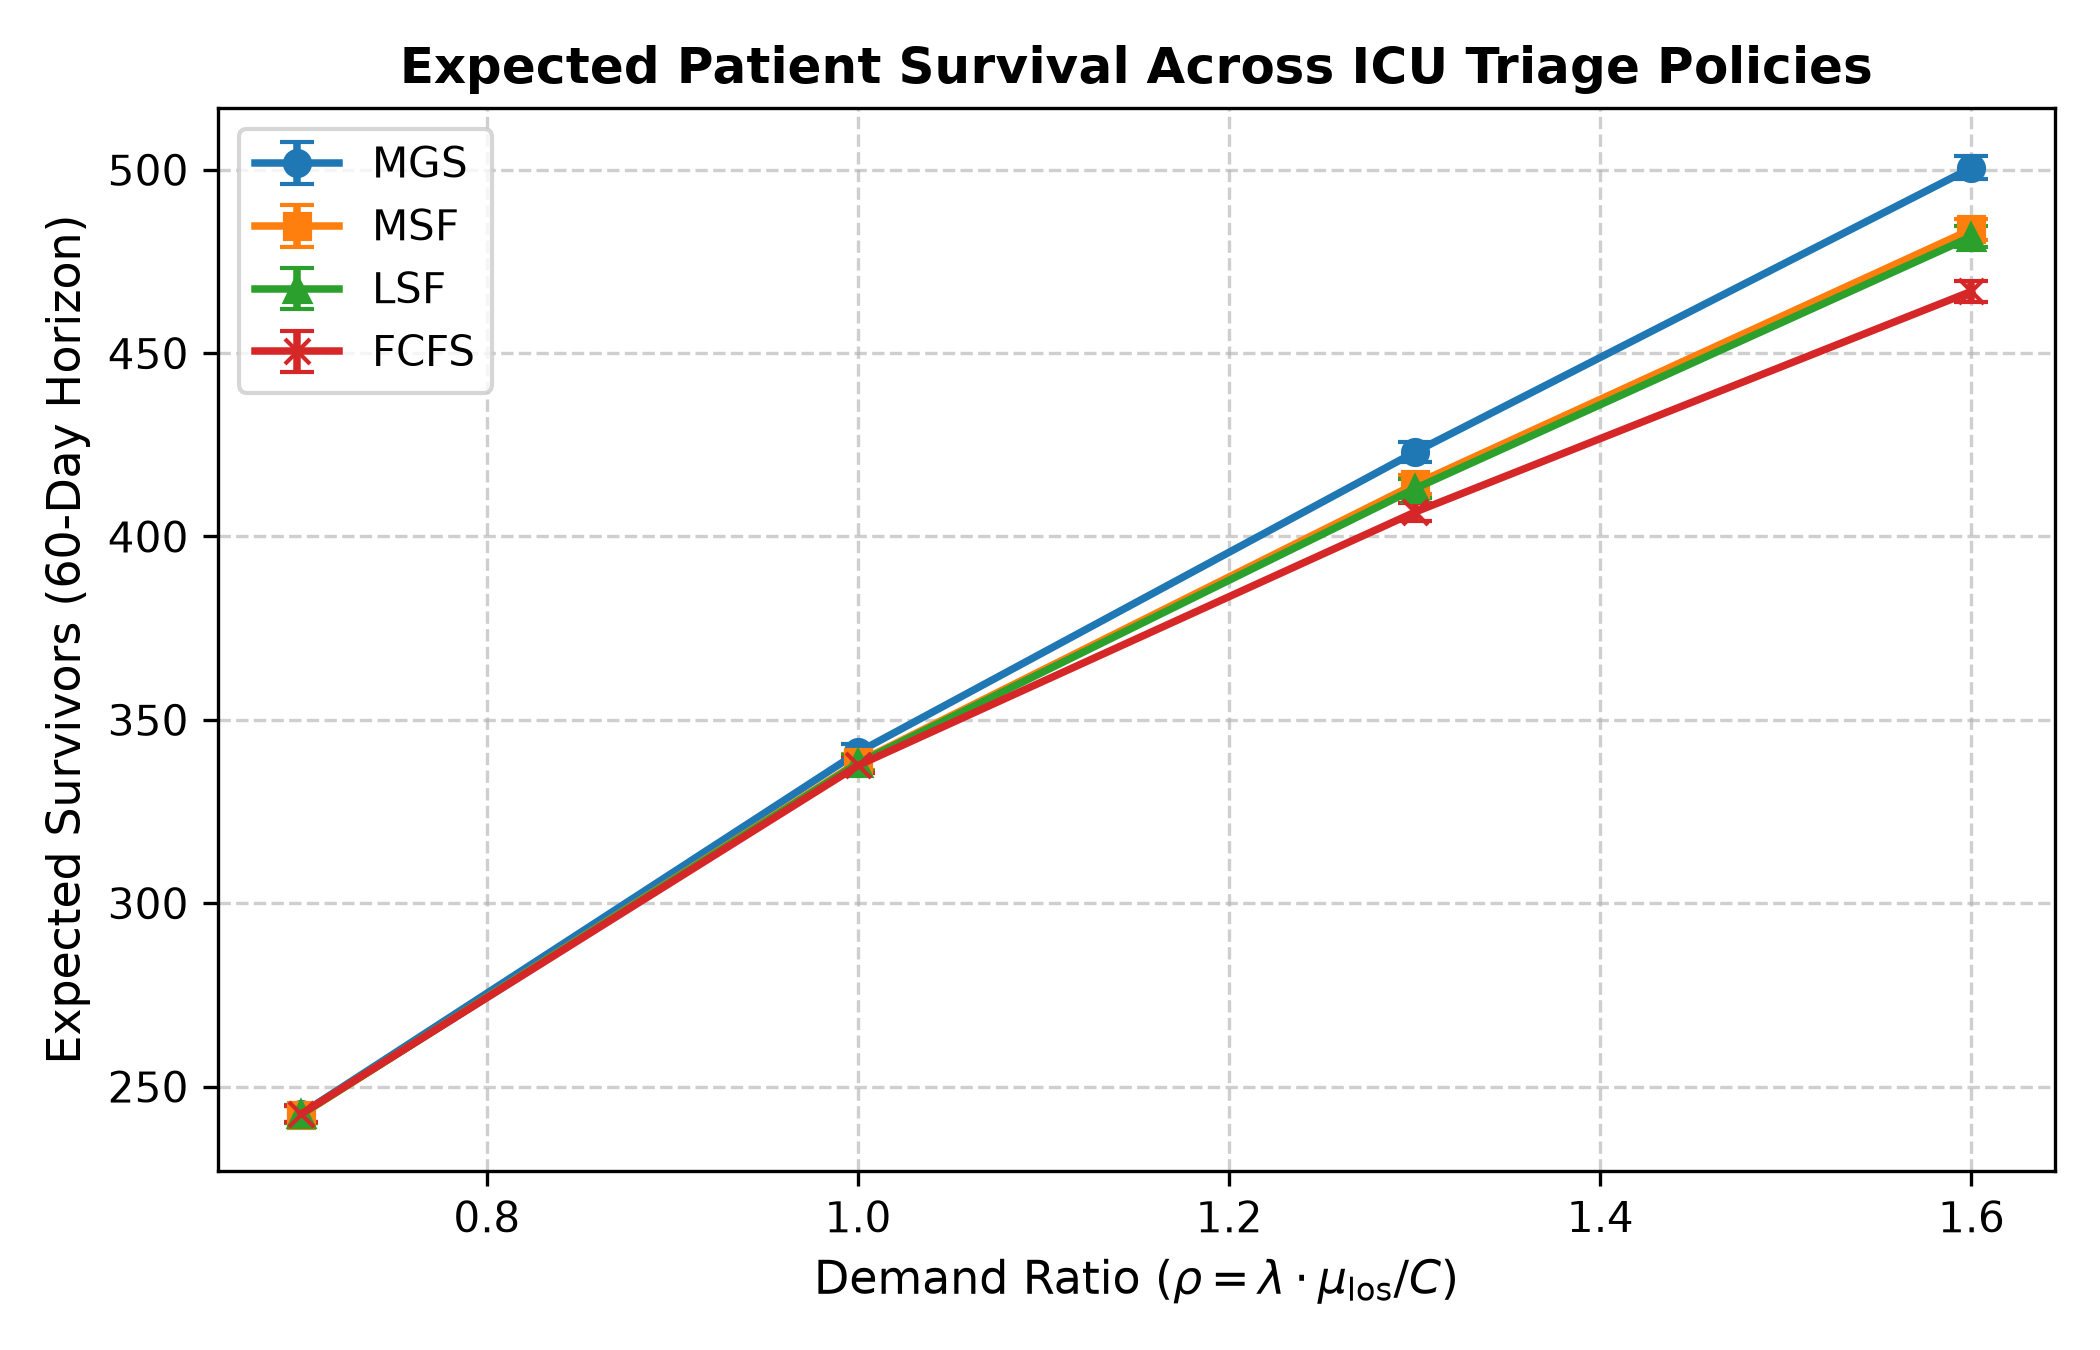
\includegraphics[width=0.85\textwidth]{fig_survivors.png}
    \caption{Expected patient survival across triage policies under increasing demand intensity (60-day horizon, 95\% confidence intervals).}
    \label{fig:survivors}
\end{figure}

\subsection{Paired Statistical Significance}

Because every replication generated an identical patient arrival sequence for all policies via Common Random Numbers, we conduct paired comparisons to evaluate the exact incremental lives saved by priority triage over the FCFS baseline (Table \ref{tab:paired_stats} and Figure \ref{fig:paired_gain}).

\begin{table}[ht]
\centering
\caption{Paired survival gain over the FCFS hospital baseline (mean $\pm$ standard error, paired $t$-statistic, and $p$-value).}
\label{tab:paired_stats}
\begin{tabular}{llccc}
\toprule
\textbf{Demand ($\rho$)} & \textbf{Policy vs. FCFS} & \textbf{Mean Lives Saved ($\Delta S$)} & \textbf{$t$-statistic} & \textbf{$p$-value} \\
\midrule
\multirow{3}{*}{\textbf{0.70}} 
 & MGS vs. FCFS & $+0.03 \pm 0.04$ & $0.71$  & $0.481$ \\
 & MSF vs. FCFS & $-0.22 \pm 0.04$ & $-5.19$ & $< 0.0001$ \\
 & LSF vs. FCFS & $-0.14 \pm 0.04$ & $-3.27$ & $0.0015$ \\
\midrule
\multirow{3}{*}{\textbf{1.00}} 
 & MGS vs. FCFS & $\mathbf{+3.60 \pm 0.21}$ & $17.51$ & $< 0.0001$ \\
 & MSF vs. FCFS & $+0.91 \pm 0.16$ & $5.54$  & $< 0.0001$ \\
 & LSF vs. FCFS & $+0.62 \pm 0.16$ & $3.86$  & $0.0002$ \\
\midrule
\multirow{3}{*}{\textbf{1.30}} 
 & MGS vs. FCFS & $\mathbf{+16.36 \pm 0.40}$ & $40.65$ & $< 0.0001$ \\
 & MSF vs. FCFS & $+7.62 \pm 0.35$ & $21.64$ & $< 0.0001$ \\
 & LSF vs. FCFS & $+6.40 \pm 0.33$ & $19.32$ & $< 0.0001$ \\
\midrule
\multirow{3}{*}{\textbf{1.60}} 
 & MGS vs. FCFS & $\mathbf{+33.67 \pm 0.47}$ & $71.68$ & $< 0.0001$ \\
 & MSF vs. FCFS & $+16.89 \pm 0.39$ & $43.31$ & $< 0.0001$ \\
 & LSF vs. FCFS & $+14.93 \pm 0.47$ & $31.57$ & $< 0.0001$ \\
\bottomrule
\end{tabular}
\end{table}

\begin{figure}[ht]
    \centering
    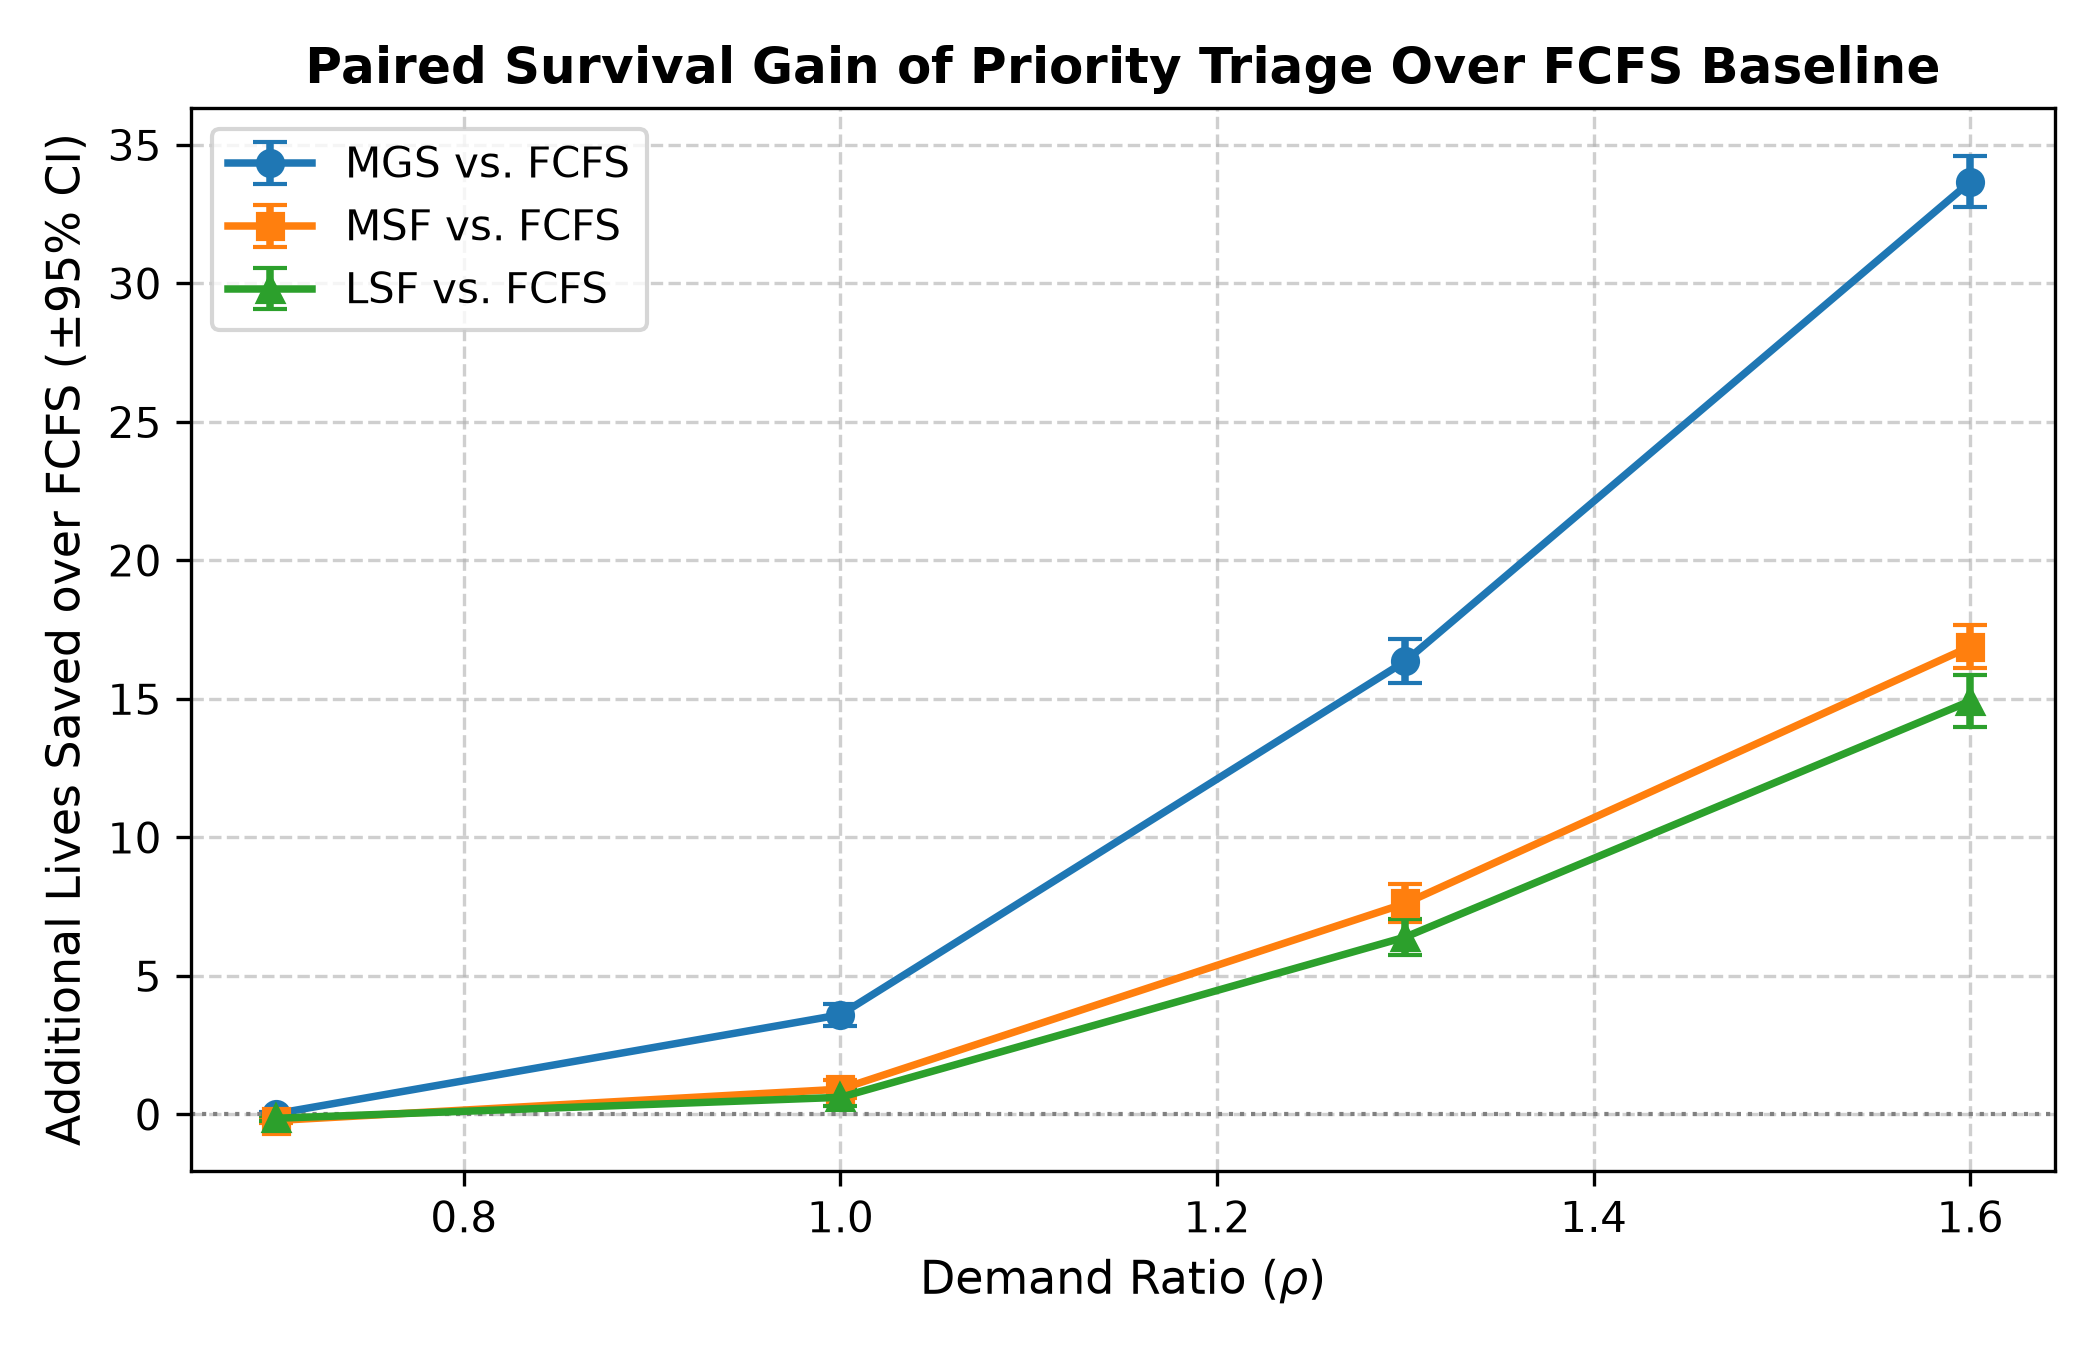
\includegraphics[width=0.85\textwidth]{fig_paired_gain.png}
    \caption{Paired additional lives saved over FCFS baseline ($\pm 95\%$ confidence intervals) across demand regimes.}
    \label{fig:paired_gain}
\end{figure}

The paired statistical evidence is conclusive:
\begin{itemize}
    \item Under severe surge ($\rho = 1.60$), MGS saves on average **$+33.67$ additional lives** over FCFS ($t = 71.68, p < 0.0001$).
    \item MGS also demonstrates clear superiority over MSF ($+16.78$ additional lives) and LSF ($+18.74$ additional lives).
    \item The mechanism behind this advantage stems directly from Eq. (\ref{eq:mgs}): MGS avoids allocating beds to patients whose condition is so irreversible that ICU admission yields minimal survival gain ($\Delta P \approx 0$), as well as patients who would survive even in general wards. Instead, beds are reserved for patients where intensive care generates the decisive therapeutic recovery.
\end{itemize}

\subsection{Queue Waiting Times and Congestion}

Figure \ref{fig:waiting_times} illustrates the impact of triage strategies on patient queue waiting times. Under low and balanced demand ($\rho \le 1.0$), queue waiting times remain moderate across all strategies ($< 12$ hours).

\begin{figure}[ht]
    \centering
    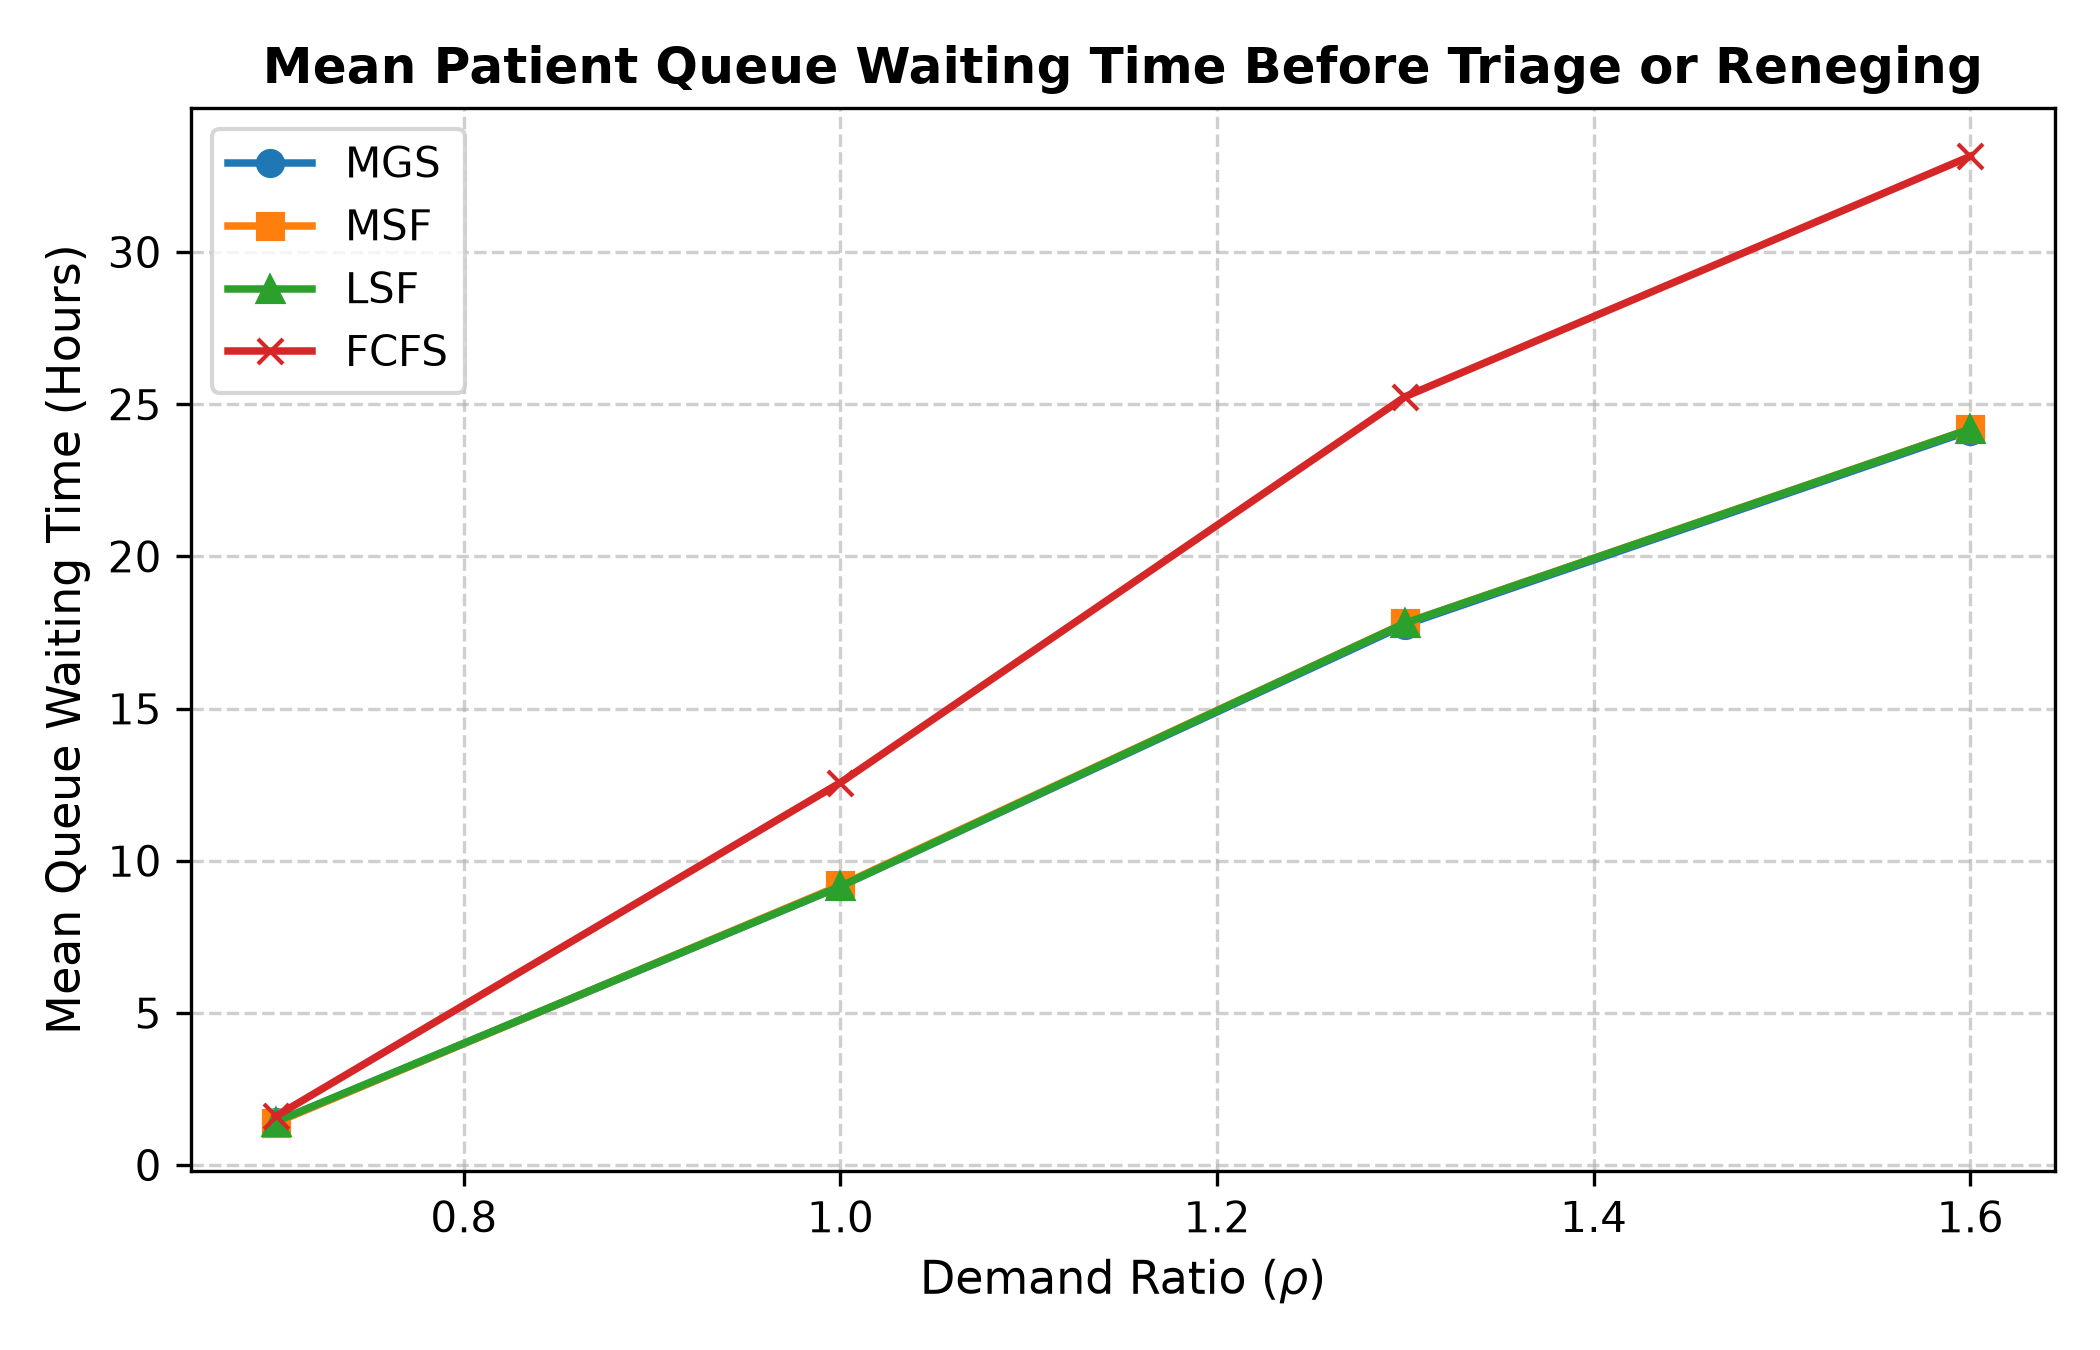
\includegraphics[width=0.85\textwidth]{fig_waiting_times.png}
    \caption{Mean queue waiting time (hours) prior to admission or reneging across demand regimes.}
    \label{fig:waiting_times}
\end{figure}

However, as demand reaches $\rho = 1.60$, FCFS causes severe queue bloat, with mean waiting times escalating to **$33.15$ hours**. In contrast, under MGS, mean waiting times are kept at **$24.13$ hours**---a reduction of over 9 hours. By selecting patients who benefit most rapidly and releasing beds efficiently, MGS mitigates queue congestion and reduces the risk of pre-ICU mortality in intermediate transit wards.

\section{Conclusions}
\label{sec:conclusion}

This paper developed a discrete-event dynamic simulation (DES) framework for allocating multi-type ICU beds under severe resource scarcity. By incorporating continuous Poisson arrivals, stochastic Log-Normal length of stay (LOS), segregated critical care categories (adult, pediatric, neonatal), and queue reneging, our model directly overcomes the limitations of static one-shot formulations identified in the literature.

The simulation was calibrated using public operational data from the University Hospital of UFMA (HU-UFMA, CNES 2024; 45 beds) and evaluated across 1,600 simulated trajectories under synchronized Common Random Numbers. The experimental results demonstrate that while triage rules are inconsequential during unconstrained demand ($\rho = 0.70$), the Maximizing Overall Survival Expectation (MGS) policy achieves statistically overwhelming advantages during surge crises ($\rho = 1.60$), preserving **$33.67$ additional lives** over conventional First-Come, First-Served hospital queues and **$16.78$ additional lives** over Most Serious First triage ($p < 0.0001$).

These findings have direct operational and ethical implications for critical care governance:
\begin{enumerate}[(1)]
    \item Hospital crisis standards of care should prioritize marginal survival gain ($\Delta P = P_{\text{in}} - P_{\text{out}}$) rather than isolated severity or chronologic arrival;
    \item Bed allocation protocols must treat adult, pediatric, and neonatal beds as specialized pools rather than aggregated capacity;
    \item Triage algorithms must be integrated into continuous electronic health record workflows that dynamically re-evaluate patient queues as beds become vacant.
\end{enumerate}

Future research directions include extending the DES engine to model dynamic nurse-to-patient staffing ratios and step-down intermediate care unit transfers.

%%-----------------------------
%%      Bibliography
%%-----------------------------
\bibliographystyle{plain}
\bibliography{bib}

\end{document}
